\chapter[Fundamentação Teórica]{Fundamentação Teórica}
\section{Sistemas Criptográficos de Chave Pública}

A proposta de chave pública foi criada a partir de dois problemas centrais. O primeiro seria o problema de distribuição de chaves, onde duas pessoas só teriam uma comunicação segura caso elas já compartilhassem uma chave anteriormente distribuída entre si. O segundo problema, que aparentemente não havia relação com o primeiro, era o problema de assinaturas digitais. Com a popularização das transações de mensagens e documentos via \textit{Internet}, viu-se a necessidade da criação de uma assinatura que fosse análoga às assinaturas convencionais. Desta maneira seria possível comprovar a outras pessoas que uma mensagem digital partiu de uma pessoa em particular. Para \citeonline[p.~560]{diffie1998} existiam duas questões sobre os problemas mencionados:

\begin{citacao}
No primeiro caso, se duas pessoas pudessem de alguma forma comunicar uma chave secreta de uma para a outra sem nunca terem se conhecido, por que não poderiam comunicar sua mensagem em segredo? O segundo não é melhor. Para ser eficaz, a assinatura deve ser impressa. Como então pode uma mensagem digital, que pode ser copiada perfeitamente, ter uma assinatura?
\end{citacao}

\citeonline{diffie1976new} descobriram uma solução para essas questões, propondo assim uma forma de duas pessoas realizarem a troca de chave por um canal não seguro, chamada de criptografia de chave pública. Essa descoberta proporcionou uma grande mudança na história da criptografia, que antes era realizada sob ferramentas elementares da substituição e permutação, e passou a ser baseada em funções matemáticas. Com essa nova descoberta passou-se a utilizar duas chaves separadas, ao invés de apenas uma chave, como era feito na criptografia simétrica \cite{stallings2014}.

Após essas descobertas, foram criados vários sistemas criptográficos de chave pública os quais providenciavam geração de chaves, algoritmos de cifração, de troca de chaves e de assinatura digital, que será discutido no próximo capítulo.

\section{Assinaturas Digitais}

O Processamento de mensagem com algoritmo de criptografia de chave pública pode oferecer a autenticação da mensagem, garantindo a origem da mensagem ao receptor e que nenhum terceiro está tentando se passar por alguma das partes. Porém, não é garantido que alguma das duas partes que trocam a mensagem realizem uma disputa. Isto poderia ocorrer caso o receptor alterasse a mensagem e alegasse que ela veio do emissor ou caso o emissor negasse a mensagem que foi enviada para o receptor. Nesses casos a autenticação não é suficiente. 

Uma solução proposta é a utilização de assinaturas digitais, provendo a autenticação da mensagem, garantindo que um emissor criou e assinou uma mensagem; a integridade da mensagem, provando que a mensagem não foi alterada após ser assinada; e o não repúdio, prevenindo que o emissor negue a autoria da mensagem \cite{johnson2001elliptic}.

É importante notar que, por conta do processo de assinatura e de verificação serem lentos devido às cifrações e decifrações, torna-se muito custosa a implementação de uma assinatura em uma mensagem por completo. Além disso, o receptor teria que armazenar o texto cifrado por completo o verificando sempre que necessário \cite{diffie1998}.

Para a solução desse problema, o processo de assinatura é baseado no resumo da mensagem, mais conhecido como \textit{hash} da mensagem, para criar a assinatura. Isso trouxe a vantagem de transmitir a assinatura independentemente da mensagem, além de permitir a criação de protocolos onde a mensagem não precisa ser transmitida, uma vez que já é conhecida por todas as partes \cite{diffie1998}.

A Figura \ref{assinaturaDigitalSimp} representa um esquema simplificado do funcionamento da assinatura digital. Para criar a assinatura de uma mensagem, deve-se passar a mensagem por uma função \textit{hash} para simplificar o processo de assinatura conforme comentado anteriormente, o resultado da função \textit{hash} é então processado com uma chave privada. Para realizar a verificação da assinatura é preciso passar a mensagem pela mesma função \textit{hash} utilizada para criar a assinatura, então esse valor junto com a assinatura digital e a chave pública são processados e uma comparação é feita a fim de validar ou não a assinatura.

\begin{figure}[h]
	\centering
	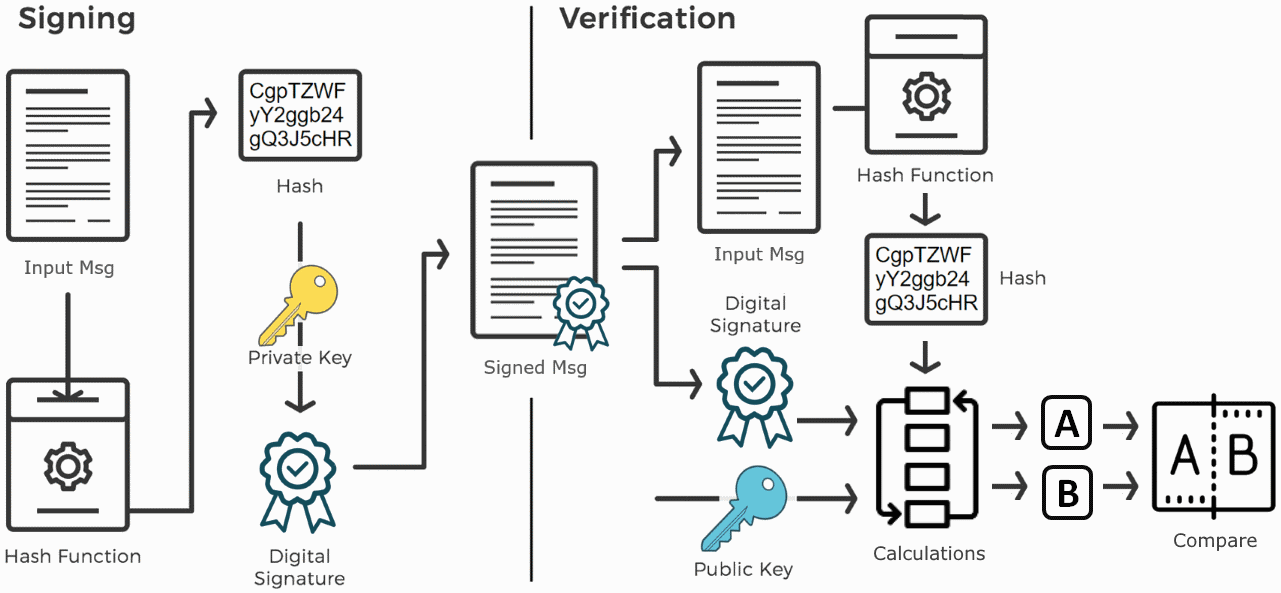
\includegraphics[keepaspectratio=true,scale=0.45]{figuras/assinatura digital.png}
	\caption{Representação simplificada dos elementos essenciais do processo de assinatura digital - Imagem retirada de \cite{nakov2018}.}
	\label{assinaturaDigitalSimp}
\end{figure}

Vários esquemas de assinatura digital foram desenvolvidos com o objetivo de garantir autenticação, integridade e não repúdio. Alguns exemplos desses esquemas são: assinaturas RSA, assinaturas ElGamal, assinaturas Schnorr, DSA, ECDSA e EdDSA. Esses dois últimos esquemas serão discutidos a seguir.

\subsection{Elliptic Curve Digital Signature Algorithm (ECDSA)}

O algoritmo de assinatura digital com curvas elípticas utiliza cálculos sob o grupo de pontos de uma curva elíptica sobre um corpo finito. Os cálculos matemáticos que geram segurança para operações com essas curvas se baseiam na inviabilidade computacional do problema do logaritmo discreto da curva elíptica (ECDLP).

Um algoritmo ECDSA deve seguir uma série de parâmetros de domínio adequados a fim de prevenir diversos ataques que poderiam comprometer a segurança do algoritmo e a detecção de codificação inadvertida ou erros de transmissão. Segundo \citeonline{johnson2001elliptic} esses parâmetros consistem em um inteiro $p$ especificando o corpo finito $\mathbb{F}_p$, dois elementos $a, b \in \mathbb{F}_p $ especificando uma curva elíptica $E(\mathbb{F}_p)$ podendo ser definida pela equação
\begin{equation}
E : y^2 = x^3 + ax + b \pmod{p},
\end{equation}
um ponto gerador $G = (x_G, y_G)$ em $E(\mathbb{F}_p)$, um primo $n$ que é a ordem de $G$, e o cofator $h = \#E(\mathbb{F}_p) / n$, onde $\#E(\mathbb{F}_p)$ é a ordem de $E$.

\subsubsection{Geração de Par de Chaves ECDSA}

Após a validação dos parâmetros de domínio da curva, ela estará apta a ser usada para gerar pares de chaves que serão necessárias para realizar assinaturas digitais.

Segundo \citeonline{johnson2001elliptic} para a geração de pares de chaves do algoritmos ECDSA primeiramente é necessário definir a chave privada, escolhendo de forma aleatória ou pseudoaleatória um inteiro $d$ no intervalo $[1, n - 1]$. A chave pública $Q$ é computada realizando a multiplicação da chave privada pelo ponto gerador $G$, e esta pode ser comprimida escolhendo uma das coordenadas e somando um bit de paridade.

\subsubsection{Assinatura ECDSA}
 
A assinatura ECDSA se baseia no esquema de assinatura de ElGamal. Para realizar a assinatura de uma mensagem $m$ é preciso seguir os seguintes passos \cite{johnson2001elliptic}:
\begin{enumerate}
    \item Escolha um número aleatório ou pseudoaleatório $k$ no intervalo $[1, n - 1]$;
    \item Calcule $kG = (x_1,y_1)$ e converta $x_1$ em um inteiro $\bar x_1$;
    \item Calcule $r = \bar x_1 \pmod{n}$;
    \item Calcule o \textit{hash} da mensagem, utilizando uma função \textit{hash} criptográfica como SHA-256 e o converta para um número inteiro $e$;
    \item Calcule $s = k^{-1} (e + dr) \pmod{n}$;
    \item A assinatura digital da mensagem $m$ se dá por ($r$, $s$)
\end{enumerate}

\subsubsection{Verificação ECDSA}

Para que seja possível verificar a assinatura ($r$, $s$) da mensagem $m$ é necessário ter conhecimento dos parâmetros de domínio da curva, assim como como a chave pública $Q$. Após isso é realizado os seguintes passos \cite{johnson2001elliptic}:
\begin{enumerate}
    \item Verificar que $r$ e $s$ estão no intervalo $[1, n - 1]$;
    \item Calcule o \textit{hash} da mensagem, utilizando uma função \textit{hash} criptográfica como SHA-256 e o converta para um número inteiro $e$;
    \item Calcule $w = s^{-1} \pmod{n}$;
    \item Calcule $u_1 = ew \pmod{n}$ e $u_2 = rw \pmod{n}$;
    \item Calcule $X = u_1 G + u_2 Q$;
    \item Se $X = \mathcal{O}$, recuse a assinatura. Caso contrário, converta a coordenada $x$ de $X$ em um inteiro $\bar x_1$ e calcule $v = \bar x_1 \pmod{n}$;
    \item Aceite a assinatura apenas se e somente se $v = r$;
\end{enumerate}

O principal objetivo na verificação da assinatura é recalcular o ponto $X$ por meio da chave pública fornecida e comparar com o ponto gerado no processo de assinatura pela multiplicação do número aleatório $k$ com o ponto gerador $G$.  

\subsection{Edwards-curve Digital Signature Algorithm (EdDSA)}

O algoritmo de assinatura digital da curva de Edwards se baseia no esquema de assinatura de Schnorr e utiliza cálculos baseado nas curvas torcidas de Edwards. Os cálculos matemáticos que geram segurança para operações com essas curvas fundamenta-se na inviabilidade computacional do problema do logaritmo discreto da curva elíptica (ECDLP).

Esse esquema de assinaturas por chave pública trás uma série de benefícios como: verificação rápida de uma única assinatura, verificação em lote ainda mais rápida, assinaturas muito rápidas, rápida geração de chaves, alto nível de segurança, chaves de sessão infalíveis, resiliência à colisões e chaves pequenas \cite{bernstein2012high}.

Assim como nos algoritmos ECDSA, é necessário uma série de parâmetros a serem seguidos com a finalidade de prevenir ataques que poderiam comprometer a segurança do algoritmo. Segundo \citeonline{bernstein2015eddsa} esses parâmetros consistem em: 
\begin{enumerate}
    \item Um expoente primo ímpar $q$ especificando o corpo finito $\mathbb{F}_q$.
    \item Um inteiro $b$ onde $2^{b-1} > q$, com a recomendação de que $b$ seja um múltiplo de 8.
    \item Uma codificação de $(b-1)$ bits dos elementos de $\mathbb{F}_q$.
    \item Uma função \textit{hash} $H$ que produza um valor de tamanho $2b$ bits, com a recomendação de se utilizar funções \textit{hash} conservativas.
    \item Um inteiro $c \in \{2,3\}$.
    \item Um inteiro $n$ onde $c \le n \le b$.
    \item Um elemento não quadrado $a$ de $\mathbb{F}_q$, com a recomendação de que $a = -1$ se $q \pmod{4} = 1$, e $a = 1$ se $q \pmod{4} = 3$.
    \item Um elemento não quadrado $d$ de $\mathbb{F}_q$.
    \item Um elemento $B \ne (0, 1)$ do conjunto $E = \big\{ (x, y) \in \mathbb{F}_q \times \mathbb{F}_q : ax^2 + y^2 = 1 + dx^2y^2 \big\}$.
    \item Um primo ímpar $l$ de tal modo que $lB = 0$ e $2^cl = \#E$.
    \item Uma função "\textit{prehash}" $H'$.
\end{enumerate}

Um exemplo de algoritmo EdDSA é o Ed25519 que utiliza a forma de Edwards edwards25519. Ed25519 utiliza uma chave privada de 32 \textit{bytes}, uma chave pública de 32 \textit{bytes} e gera uma assinatura de 64 \textit{bytes}. Seus parâmetros consistem em:

\begin{enumerate}
    \item Um primo $ q = 2^{255} - 19$.
    \item $b = 256$.
    \item A codificação 255 bits de $\mathbb{F}_{2^{255}-19}$ é a codificação \textit{little-endian} em $\{ 0,1,..., 2^{255}-20 \}$.
    \item A função \textit{hash} utilizada é a SHA-512;
    \item $c = 3$.
    \item $n = 254$.
    \item $a = -1$ pois $q \pmod{4} = 1$.
    \item $d = -121665/121666$
    \item $B$ é o ponto $(...202, 4/5) \in E$.
    \item $l$ é o primo $2^{252} + 27742317777372353535851937790883648493$.
    \item $H'$ é a função identidade, ou seja, $H'(M) = M$
\end{enumerate}

\subsubsection{Geração de Par de Chaves EdDSA}

Com os valores dos parâmetros de domínio da curva escolhidos e validados, é possível gerar pares de chaves que serão utilizados para assinar mensagens e verificar assinaturas digitais.

Segundo \citeonline{bernstein2015eddsa}, a chave privada $k$ é um número aleatório de tamanho $b$ bits. A função \textit{hash} $H(k) = (h_0,h_1,...,h_{2b-1})$ determina um inteiro $s = 2^n \sum_{c \le i < n} 2^ih_i$ que por sua vez determina o múltiplo $A = sB$, onde \underline{A} é a chave pública.

\subsubsection{Assinatura EdDSA}

O algoritmo de assinatura EdDSA utiliza uma mensagem $M$ e uma chave privada $k$. Dessa forma define-se $r = H(h_b, ..., h_{2b-1}, M) \in \{ 0, 1, ..., 2^{2b} - 1 \}$; $R = rB$; $S = (r + H(\underline{R}, \underline{A}, M)s) \pmod{l}$. A assinatura de $M$ sob $k$ é o par de inteiros $(\underline{R}, \underline{S})$ de tamanho $2b$ bits, onde \underline{R} possui um ponto comprimido e um inteiro \underline{S} que indica que o assinante conhece a chave privada $k$ e a mensagem $M$  garantindo o não repúdio \cite{bernstein2015eddsa}.

No esquema de assinatura ECDSA, é necessário realizar a criação do valor $r$ para cada mensagem de forma aleatória. Caso $r$ seja o mesmo para duas mensagens então a chave privada poderá ser descoberta \cite{ElGamalCrypto}. Um caso concreto dessa falha ocorreu no esquema de assinatura ECDSA implementado para a assinatura de código do console PlayStation3 da empresa Sony \cite{ps32010}.

Para evitar esse problema, o algoritmo EdDSA gera um valor de $r$ dependente da mensagem, resultando em um $r$ diferente para cada mensagem assinada.

\subsubsection{Verificação EdDSA}

A verificação é feita utilizando a mensagem $M$, a chave pública do assinante $\underline{A}$ e a assinatura $(\underline{R}, \underline{S})$. Primeiramente recuperam-se os pontos da curva elíptica $A$ e $R$ dos pontos comprimidos $\underline{A}$ e $\underline{R}$. Depois calcula-se $H(\underline{R}, \underline{A}, M)$ e verifica-se o grupo de equação $2^cSB = 2^cR + 2^cH(\underline{R}, \underline{A}, M)A$ em $E$. A assinatura deve ser rejeitada caso a recuperação dos pontos falhe ou se a comparação divergir. 
